\newpage
\appendix
\chapter{Apêndice 2}
\label{apendice2}

\section{Descrição de testes de aceitação}

Essa estrutura é proposta da seguinte forma:

\begin{enumerate}
\item \textbf{Título:} Palavra-chave ‘\textit{feature}’ e um título curto que representa o 
objetivo da \textit{feature}.
\item \textbf{Narrativa:} um texto curto que demonstre os cenários de execução, 
exatamente como a narrativa de uma história de usuário:

\begin{figure}[!h]
    \centering
    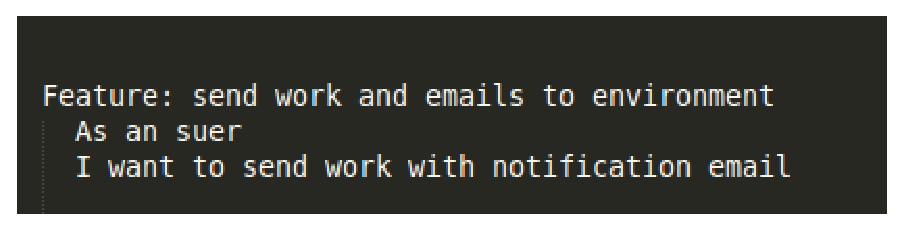
\includegraphics[keepaspectratio=true,scale=0.50]
      {figuras/noosfero_feature2.eps}
    \caption{Descrição do título (\textit{feature}) de um teste}
    \label{nosfero_feature}
\end{figure}

\item \textbf{Pré condições:} representado pela palavra-chave \textit{'background'}, define os passos 
precedem cada cenário de teste.

\begin{figure}[!h]
    \centering
    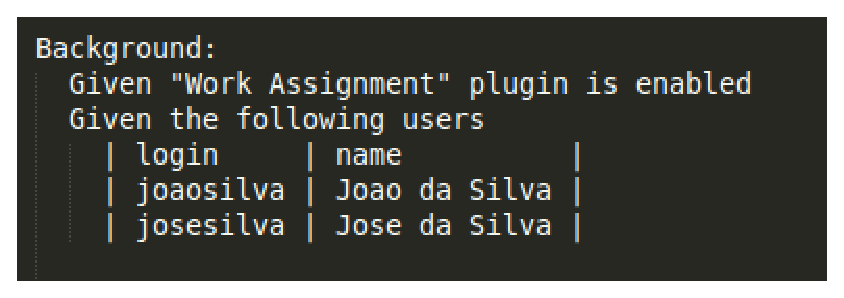
\includegraphics[keepaspectratio=true,scale=0.50]
      {figuras/noosfero_back.eps}
    \caption{Descrição de pré condições (\textit{background}) de um teste}
    \label{nosfero_feature}
\end{figure}

\item \textbf{Cenários:} representam parte concreta de como o software deve se 
comportar, e sendo a parte essencial do teste realizado no 
cucumber. Após a palavra-chave \textit{‘scenario’} define-se o nome do cenário em questão:
\item \textbf{Passos:} Cada cenário possui uma série de passos que demonstram o seu 
comportamento, que são linhas simples iniciadas com as seguintes palavras-chaves: 
\textit{Given, When, Then, And, But}.
\item \textbf{Given:} Indica uma condição inicial para que o cenário seja executado, 
trata-se das pré-condições do cenário.
\item \textbf{When:} Indica o evento do cenário
\item \textbf{Then:} Indica o que é esperado após o evento ocorrer.

\begin{figure}[!h]
    \centering
    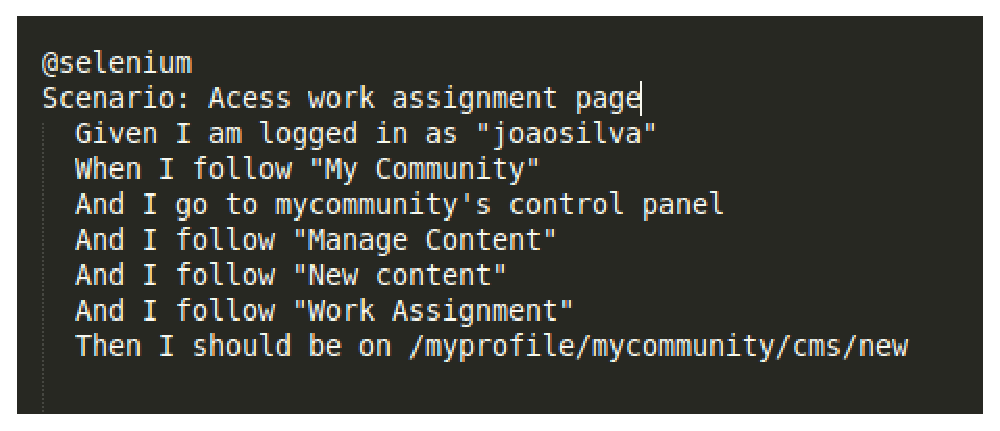
\includegraphics[keepaspectratio=true,scale=0.50]
      {figuras/noosfero_scenario.eps}
    \caption{Descrição do cenário (\textit{scenario}) de um teste}
    \label{nosfero_scenario}
\end{figure}

\end{enumerate}

\section (Descrição de funcionais e unitários)

Os testes funcionais e unitários são escritos da seguinte forma:

\textbf{Setup:} indica as condições inciais dos testes, setando variáveis de ambiente e de configuração por exemplo.

\begin{figure}[!h]
    \centering
    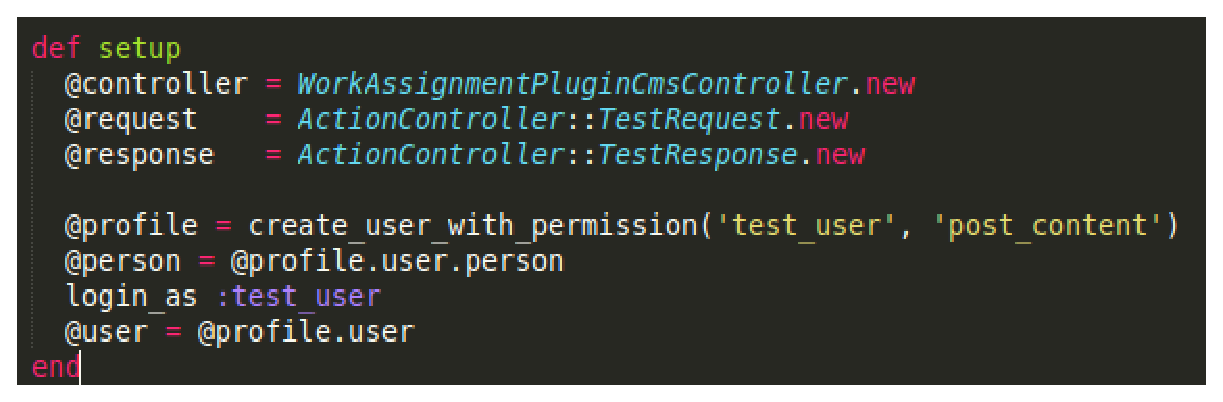
\includegraphics[keepaspectratio=true,scale=0.5]
      {figuras/teste_setup.eps}
    \caption{Descrição do setup de um teste}
    \label{nosfero_setup}
\end{figure}

\textbf{Título:} título do teste iniciado com a palavra \textit{‘should’} e finalizado com \textit{‘do’}

\textbf{Passos:} código que define o comportamento do teste

\textbf{Verificação:} Assertiva que verifica se a ação foi realizada como esperada.

\begin{figure}[!h]
    \centering
    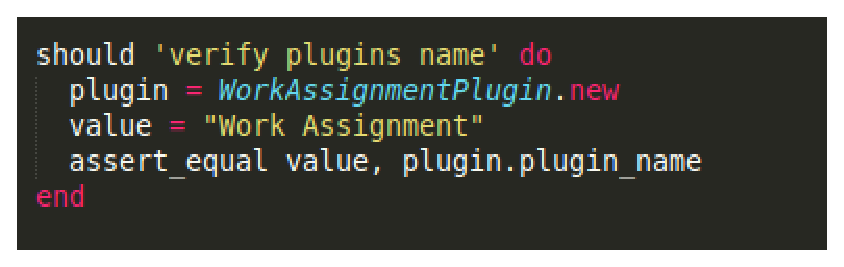
\includegraphics[keepaspectratio=true,scale=0.55]
      {figuras/teste_should.eps}
    \caption{Código de teste}
    \label{noosfero_should}
\end{figure}